\documentclass{article}
\usepackage[T1]{fontenc}
\usepackage[utf8]{inputenc}
\usepackage[margin=1in]{geometry}
\usepackage{amsmath}
\usepackage{graphicx}

\newcommand{\HRule}{\rule{\linewidth}{0.5mm}}
\newcommand{\Hrule}{\rule{\linewidth}{0.3mm}}

\title{Lab Report 3}
\author{Yuhuang Chen (804449266), Zeyuan Xu (004255573)}
\date{}


\begin{document}
  \maketitle% prints the title block
  \thispagestyle{empty}

\section{Part 1: MicroBlaze Hello World}
This part of the lab aims to introduce us to using Microblaze soft processor on FPGA board. The process is simply going through the complicated GUI environment of Xilinx EDK and SDK and deploy a Hello World project. Not much is required for reporting of this part: it is all about learning the GUI and going through the most basic process of deploying C program on the soft processor. 

\section{Part 2: Serial Multiplication}
In this part, we managed to transfer strings between PC serial terminal and the Microblaze CPU, the connection is enabled by the serial connection on FPGA board. The transfer is done via the C language's STDOUT and STDIN. 
\subsection{Introduction and Source Code}
This part is simply to specify two digits as serial input, and output their product as the serial output. The computation is done on the FPGA. If the two numbers' product exceeds 100, an LED would also blink. This is done by specific mapping in the UCF file and calling the function \begin{verbatim}
LED(XPAR_LEDS_8BIT_DEVICE_ID,8);
\end{verbatim}
The source code is in C and fairly straightforward, as shown below: 
\begin{verbatim}

#include <stdio.h>
#include "xparameters.h"
#include "xil_cache.h"
#include "xbasic_types.h"
#include "xgpio.h"
#include "gpio_header.h"
#include "uartlite_header.h"
#include "xuartns550_l.h"
#include "xuartns550_l.h"
#include "uartns550_header.h"
#include "platform.h"

int main()
{
    init_platform();


    int a,b,a_sign,b_sign;
    char c;
    int operand;

    a = 0;
    b = 0;
    a_sign = 1;
    b_sign = 1;
    operand = 0;
    xil_printf("Input format: a*b\n");

    fflush(stdout);
    while((c = getchar()) != '\n') {
    	if(c == 0) {
    		continue;
    	}
    	if(c == '*') {
    		operand = 1;
    		continue;
    	}
    	if(c == 13){
    		continue;
    	}
    	if(c == '-'){
    	    if(operand == 0){
    	    	a_sign *= -1;
    	    }
    	    else{
    	    	b_sign *= -1;
    	    }
    	    continue;
    	}
    	if(c < '0' || c > '9'){
    		xil_printf("Input not expected %d\n", c);
    		return 0;
    	}
    	if (operand == 0){
    		a = a * 10;
    		a = a + c - 48;
    	}
    	else {
    		b = b * 10;
    		b = b + c - 48;
    	}
    }
    xil_printf("a   = %d\n", a*a_sign);
    xil_printf("b   = %d\n", b*b_sign);
    xil_printf("a*b = %d\n", a*b*a_sign*b_sign);

    if(a*b*a_sign*b_sign > 100) {
    	LED(XPAR_LEDS_8BIT_DEVICE_ID,8);
    }

    return 0;
}
\end{verbatim}

\subsection{Difficulties Encountered}
The difficulties mainly come from the carriage returns and null-bytes arbitrarily introduced by the serial connection. This messed up with the inputs and we have to explicitly handle these readings as exceptions (as shown in the source code). Another difficulty comes from the serial connection in Putty, as it sometimes randomly hangs and receives no inputs. The problem is resolved after we stick with the terminal in the SDK. 


\section{2.b: Rock Paper Scissor}
\subsection{Introduction and Source Code}
in this part, we need to simulate two players in the rock paper scissor game. The two players are specified as PC's keyboard input and a keypad device connected to the FPGA. We need to treat both as serial inputs, and handle the hardware mapping of keypads to pins of FPGA. The schematic diagram of the keypad is shown in figure 1, and the mapping to GPIO is done through...

\begin{figure}[h]
  \centering
  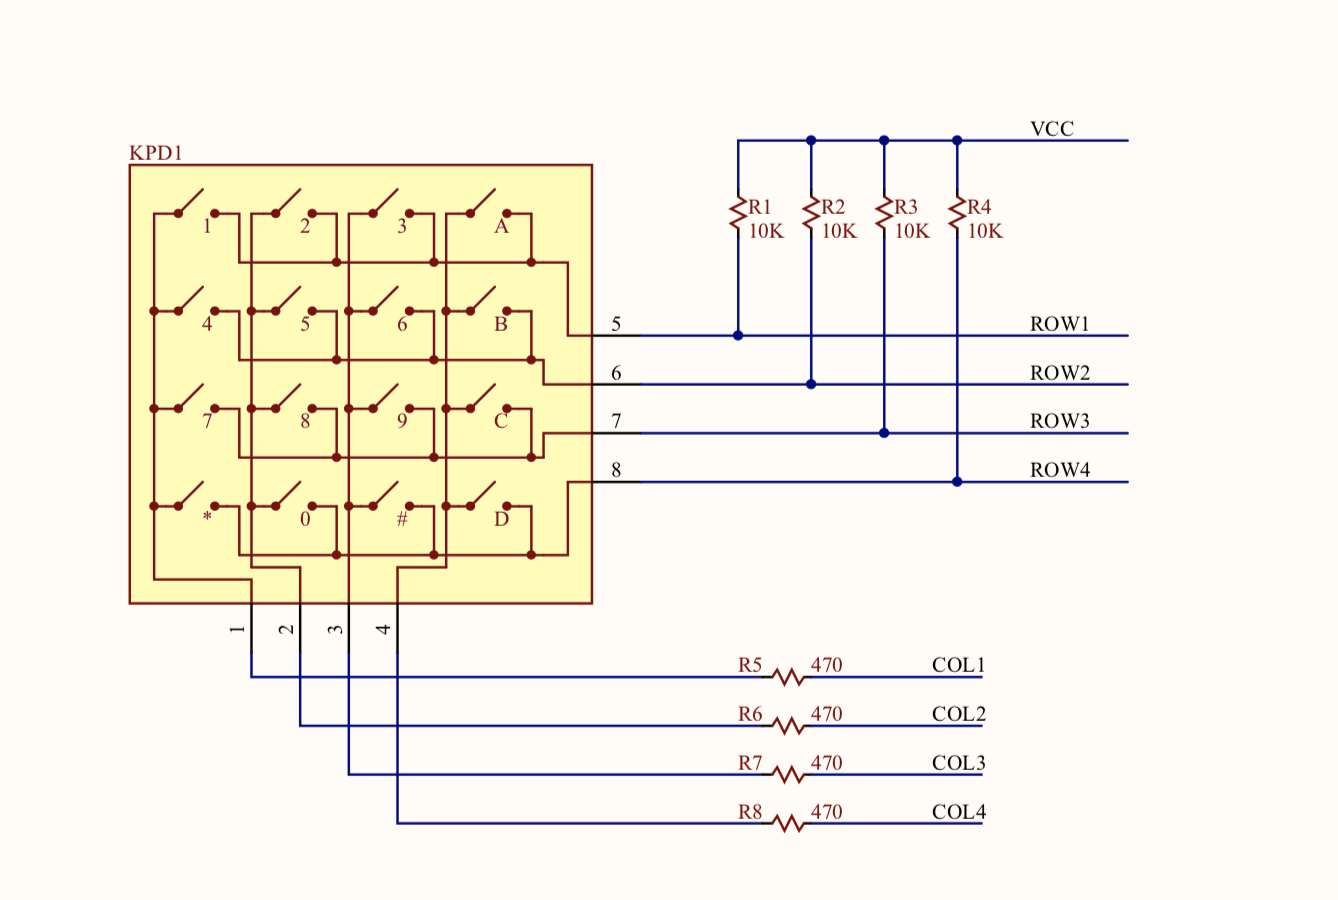
\includegraphics[width=\linewidth]{schematics.png}
  \caption{Schematics of Keypad}
  \label{fig:schematics}
\end{figure}

The C source code is shown below. It handles the serial I/O and the game logic: 
\begin{verbatim}

#include <stdio.h>
#include "xparameters.h"
#include "xil_cache.h"
#include "xbasic_types.h"
#include "xgpio.h"
#include "gpio_header.h"
#include "uartlite_header.h"
#include "xuartns550_l.h"
#include "xuartns550_l.h"
#include "uartns550_header.h"
#include "platform.h"

#define KEYPAD_CHANNEL 1

int main() 
{

	init_platform();

	char pc, fpga;
	char c;
	int Status;
	int DeviceId = XPAR_KEYPAD_DEVICE_ID;

	u32 Data = 0;
	u32 OldData = 0;

	XGpio Gpio;
	XGpio Led;
	XGpio Sw;

	Status = XGpio_Initialize(&Gpio, DeviceId);
	if (Status != XST_SUCCESS)  {
		return XST_FAILURE;
	}

	XGpio_SetDataDirection(&Gpio, KEYPAD_CHANNEL, 0x0f);


	while(1){
		xil_printf("Begin\n");
		pc = 0;
		fpga = 0;

		xil_printf("PC\n");
		while((c = getchar()) != '\n') {
		    if(c == 0 || c == 10 || c == 13) {
		    	continue;
		    }
		    if(pc == 0){
		    	pc = c;
		    }
		    else{
		    	xil_printf("Ignoring the rest of characters.\n");
		    }
		}

		xil_printf("FPGA\n");
		while(fpga == 0) {
			XGpio_DiscreteWrite(&Gpio, KEYPAD_CHANNEL, 0x70);
			Data = XGpio_DiscreteRead(&Gpio, KEYPAD_CHANNEL);
			if(Data == 0x7F){
				continue;
			}
			if(Data == 0x7E) {
				fpga = 'r';
			}
			else if(Data == 0x7D) {
				fpga = 'p';
			}
			else if(Data == 0x7B) {
				fpga = 's';
			}
			else{
				fpga = 'd';
			}
		}


		if(pc == 'p' && fpga == 'p'){
			xil_printf("Tie! PC paper = FPGA paper \n");
		}
		else if(pc == 'p' && fpga == 'r'){
			xil_printf("PC won! PC paper > FPGA rock \n");
		}
		else if(pc == 'p' && fpga == 's'){
			xil_printf("FPGA won! PC paper < FPGA scissors \n");
		}
		else if(pc == 'r' && fpga == 'p'){
			xil_printf("FPGA won! PC rock < FPGA paper \n");
		}
		else if(pc == 'r' && fpga == 'r'){
			xil_printf("Tie! PC rock = FPGA rock \n");
		}
		else if(pc == 'r' && fpga == 's'){
			xil_printf("PC won! PC rock > FPGA scissors \n");
		}
		else if(pc == 's' && fpga == 'p'){
			xil_printf("PC won! PC scissors > FPGA paper \n");
		}
		else if(pc == 's' && fpga == 'r'){
			xil_printf("FPGA won! PC scissors < FPGA rock \n");
		}
		else if(pc == 's' && fpga == 's'){
			xil_printf("Tie! PC scissors = FPGA scissors \n");
		}
		else{
			xil_printf("Unknown Input PC %c FPGA %c\n", pc, fpga);
		}
	}

   return 0;
}
\end{verbatim}

\subsection{Difficulties Encountered}
The difficulties are mainly with the Keypad mapping and GPIO configurations. After searching online about the schematics of the keypad, we solved it by: ... 

\section{Summary}
In conclusion, in this lab we finished the basic tutorials of the EDK and SDK development and become comfortable dealing with peripheral device I/O and serial communication through Microblaze. most importantly, we learned to use soft processor technology and develop FPGA projects in C code. 



\end{document}